\section{Docker image}
\label{sec:intro:docker_image:docker_img}
In this section, the Docker image is explained in more detail, as it is an important part of the work. First, the architecture of a Docker image is presented with the necessary information for further work, since the overall architecture with all information would make the basic chapter too large. Then the construct for building a Docker image is explained. This is called Dockerfile and in the introduction the key factors and usage of Dockerfile is explained. 
Finally, the last subsection describes the metadata information, as it is important to follow the theoretical concept.

\subsection{Docker Image architecture}
\label{sec:intro:docker_image:docker_img:architecture}
A Docker image is ultimately a stack of selected file system layers to provide a starting point for a container.
Fig \ref{sec:intro:docker_image:docker_image_stack} shows how a Docker image is stacked. At the bottom there is the Linux kernel. On top of that takes two different image layers place. In this case it is a Debian and a Busybox.
Both of them are runnable base images.
On top of these layers can be more layers stacked as shown on the Debian layer with an additional Emacs and an Apache layer. The busybox itself doesn't have another further layer stacked on the top.
When a container is launched from an image, Docker finally attaches a read/write file system across all underlying layers, as it is seen on both images in this example.

\begin{figure}[htbp]
 \centering
 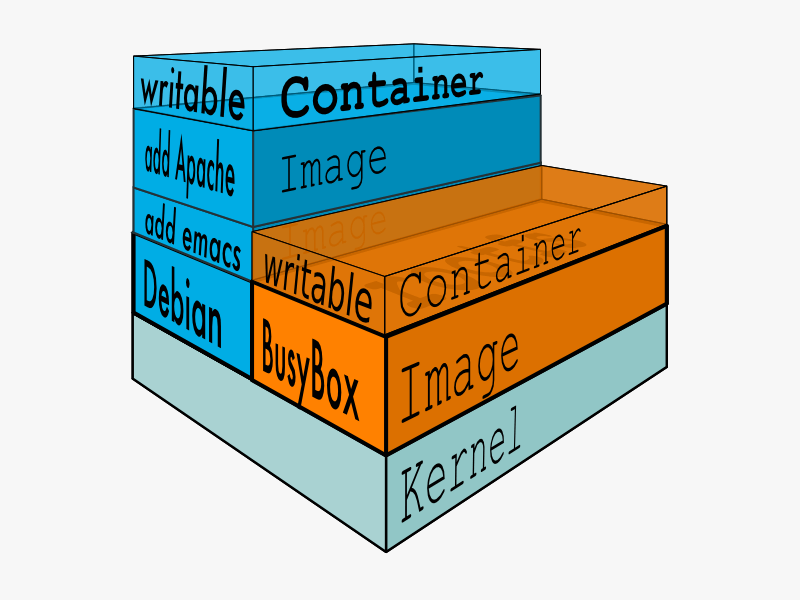
\includegraphics[width=0.6\textwidth]{gfx/examples/docker-filesystems-busyboxrw}
 \caption{Docker filesystems stacked to represent an image}
\label{sec:intro:docker_image:docker_image_stack}
\end{figure}

In order to manage images and especially corresponding file system layers, Docker uses storage drivers. Each storage driver handles the implementation differently.
There are several storage drivers available like, ZFS, BTRFS and many more which can be configured by the responsible system-engineer or developer. Docker uses in the latest version Overlay2 as storage driver per default. The Overlay2 informations about an image can be viewed by the Docker inspect command.
\begin{lstlisting}
	docker inspect ubuntu
\end{lstlisting}

The inspection provides a result tailored to show only filesystem level information, as this is the interesting part for the docker architecture.
 
\lstinputlisting[caption={Docker inspection results}, firstline=71, lastline=79, captionpos=b, label={sec:intro:docker_image:corresponding_unionfs}]{chapters/intro/listings/inspect_results.txt}

As seen in listing \ref{sec:intro:docker_image:corresponding_unionfs}, the introduced mechanisms of the Overlay2 union file system \ref{sec:intro:docker_image:unionfs} are used in order to provide a starting point for a container.
Each component of Overlay2 is found and is used by Docker. This represents once more, that Docker is using only Linux well known core functions instead of building own mechanisms.

One interesting and important fact is the mount process. The lower-directories which represents a readonly structure are not mounted directly by their folder name. Docker uses for each image layer a symbol link, which redirects to the original folder. The reason belongs only to the length of the folder name, which is in total a length of 65. These symbolic links help avoid the Linux ‘mount’ command from exceeding page size limitation.
It is also important to note that the \textbf{diff} directory in each layer builds the chain of the overlay. That can be seen in listing \ref{sec:intro:docker_image:corresponding_unionfs} as well. In each layer are additional helper files available like the lowerfile, which creates a relation to associated parent, if a parent exist.
The lower files are responsible for creating the correct order from the most upper layer to the lower layers. Due to this fact will be a correct order provided, since it is necessary for a correct behavior of a union file system.

Furthermore, every image has a name and a tag. An image name is made up of slash-separated name components, optionally prefixed by a registry hostname. The hostname must comply with standard DNS rules, but may not contain underscores. A tag name must be valid ASCII and may contain lowercase and uppercase letters, digits, underscores, periods and dashes. A tag name may not start with a period or a dash and may contain a maximum of 128 characters.
It is important to know that the name and the tag are separated by a colon.
This knowledge about the naming and tagging connection is helpful, since it finds application in the following chapters. The next section describes the construct of building a Docker image, called Dockerfile.

\subsection{Dockerfile}
\label{sec:intro:docker_image:docker_img:dockerfile}
In order to build a Docker image, Docker Inc. introduced a construct called Dockerfile.
Each entry in this Dockerfile starts with a keyword. These keywords can be used by a developer to assemble an image. Each entry in a Dockerfile creates a different file system layer. In other words each file system layer represents an instruction with help of a keyword in a Dockerfile.
The Dockerfile construct provides around 20 keywords \cite{dockerfile_ref}.
The following listing in \ref{sec:intro:docker_image:dockerfile} shows a typical Dockerfile.
\lstinputlisting[caption={Dockerfile}, captionpos=b, label=sec:intro:docker_image:dockerfile]{chapters/intro/listings/dockerfile.txt}
The FROM statement starts out by creating a layer from the ubuntu:18.04 image. The COPY command adds an example bash script from the Docker client’s current directory. The RUN command makes the program executable. Finally, the last layer specifies which command will be executed inside the container.

An image can be created with the corresponding Dockerfile and the command Docker build, like it is shown below.
\begin{lstlisting}
	docker build <my_new_image> -f <dockerfile>
\end{lstlisting}
It is valuable to know the Dockerfile construct, because it is finally responsible for integrating secrets into an image. 
From a logical view, there are two categories in a Dockerfile which contain commands that are responsible for integrating static files.
First, \textit{direct integration} which contains the actions COPY and ADD. The difference between the two commands lies in the range of functions. ADD can as an example request an URL or unzip an archive directly to the endpoint.

The second category \textit{indirect integration} is a bit more comprehensive. This category contains the action RUN.
Docker itself uses RUN to trigger a shell command and commit it to a new image layer.
The executed shell commands for RUN are inline defined. That allows cases, loop-constructs and external program execution. A flexible bunch of code is allowed, since it is just standard bash. This allows a developer to use available tools like ssh-keygen, openssl and manual file and folder creation. It is totally up to the developer what do to with that inline command in the Dockerfile. 


At this time it is known what a Docker image is and how it can be built. Also, it is known to integrate static files into an image in an indirect and direct way.  The next subsection will introduce the important topic metadata of an image which will be definitely used in the following chapters. 

\subsection{Docker Metadata}
\label{sec:intro:docker_image:docker_img:meta}
Another important feature is the metadata of an image. Every Docker image contains several meta-information of the build process. These meta-informations are directly accessible through the history feature. 
These informations are locally provided and accessible for the root user. 
It is assumed in this work that no manipulation of the metadata was performed locally. An integrity check would be desirable and need further investigation.

Using Ubuntu 18.04 as an example, the meta-information looks like this below \ref{sec:intro:docker_image:meta}:
\lstinputlisting[caption={Prototype structure in Python}, captionpos=b, label={sec:intro:docker_image:meta}]{chapters/main/practical/listings/meta.txt}
This listing might be confusing but it is helpful to just get an overview how it is structured, and how it can be helpful for the next chapters.
It can be seen that the schema of this meta information is similar to JSON. The only difference is that numeral values are not marked in quotations. In this structure there are many attributes with their corresponding values. Attributes like "Created", "CreatyBy" are first followed by "Id" and many more. 	
Important informations are most of all Dockerfile instructions like COPY, ADD an RUN, since they are responsible for integrating static files into the image.
In this example it can be seen that only an ADD command is used. A COPY method is not used.
A special fact applies to the RUN command. RUN commands are not directly listed in the meta informations.
Instead, only the executable command that follows a RUN command is visible.

In theory it is easy to analyse these informations because it is readable for computers because of the javascript object notation similarity.
That makes this history feature of Docker very important especially when it comes to the (pre-)processing of Docker images.	 Important properties can be extracted, such as Dockerfile keywords and corresponding parameters.

This chapter provided a basic knowledge about the architecture Docker images and the interaction with Overlay2. This knowledge is fundamental to have an idea how the file structure is working behind the scenes. It gives some ideas for the theoretical concept to analyse such an image for static secrets.
Before this is possible some related work is shown about key leak techniques. Key leak techniques are essential in order to detect secrets.